% -*- coding: utf-8 -*-
This chapter provides some examples which are planned to guide GMES users. Most of the examples can be found at the source code release of GMES\index{GMES}. These examples are compatible on version 0.9.5 of GMES\index{GMES}.

\section{Two-dimensional TM$_z$ cylindrical-wave propagation in air}
The first example is a simulation of a cylindrical wave which propagates in a 2-dimensional free space. In the case of 2 and 3-dimensional simulation, we can use lighter version of \texttt{FDTD} class. The code in figure \ref{fig:air2d_code} uses a class for two-dimensional transverse-magnetic mode with respect to $z$ (TM$_z$), \texttt{TMzFDTD} class. To initialize the \texttt{TMzFDTD} class, at least three parameters are required; \texttt{space}, \texttt{geom\_list}, and \texttt{src\_list}.

The \texttt{space} parameter of the \texttt{TMzFDTD} class is to define the coordinate of the calculation domain. Though GMES will supports various coordinate system in the future, the current version of GMES only supports Cartesian coordinates. A two-dimensional open space is made by the \texttt{Cartesian} class with 0 size to the $z$ dimension. The geometrical configuration is set by the second parameter, \texttt{geom\_list} of the \texttt{TMzFDTD} class. The whole domain is wrapped by the ABC\index{ABC} to absorb the outgoing waves without reflection. This space is filled with air by placing a \texttt{DefaultMedium} object\index{DefaultMedium class} consisting of \texttt{Dielectric} object\index{Dielectric class} with default parameters. A source with $E_z$ component which oscillates sinusoidally is represented using \texttt{Continuous}\index{Continuous class} and \texttt{PointSource} objects\index{PointSource class} located at the center of the space.

\begin{figure}[hp!]
  \centering
  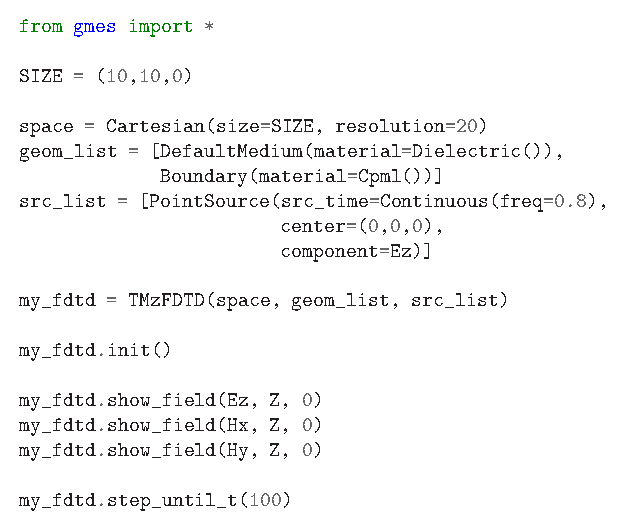
\includegraphics{figure/air2d}
  \caption{Example of 2-D TM$_z$ cylindrical-wave propagation}
  \label{fig:air2d_code}
\end{figure}

A simple on-time visualization display will show the $E_z$, $H_x$, and $H_y$ fields of the outgoing wave distributed within the grid, as shown in figure \ref{fig:air2d_field_view}. You can compare the spatial-symmetry properties of these fields with respect to the center of the space where the excitation is applied. As shown this example, the field display\index{field display} is useful to check the correct working of the simulation.

\begin{figure}[hp!]
  \begin{center}
    \subfigure[]{
      \includegraphics[width=0.45\textwidth]{figure/air2d_ez}
      \label{fig:air2d_ez}
    }
    \subfigure[]{
      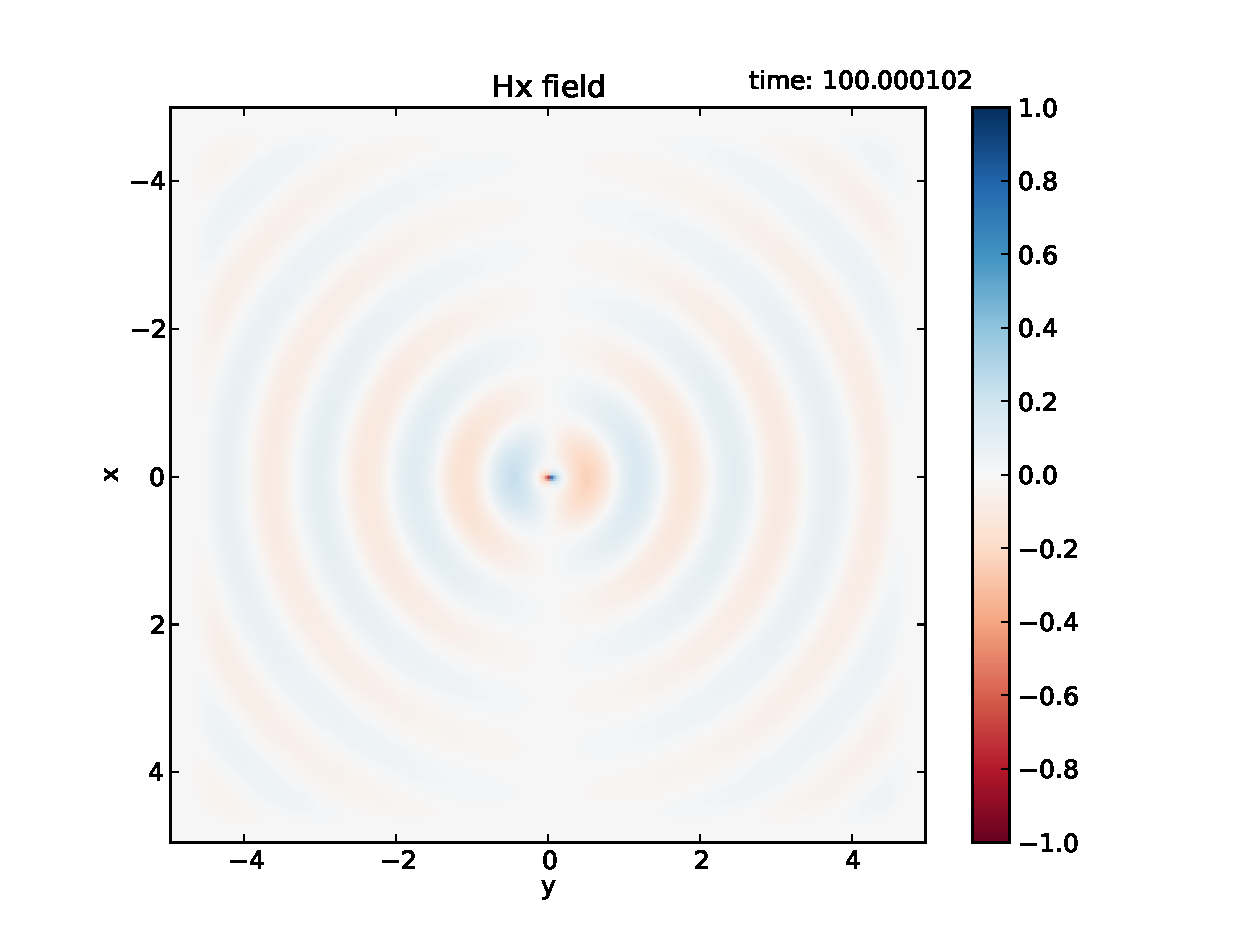
\includegraphics[width=0.45\textwidth]{figure/air2d_hx}
      \label{fig:air2d_hx}
    }
    \subfigure[]{
      \includegraphics[width=0.45\textwidth]{figure/air2d_hy}
      \label{fig:air2d_hy}
    }
  \end{center}
  \caption{Field displays of (a) $E_z$, (b) $H_x$, and (c) $H_y$ components}
  \label{fig:air2d_field_view}
\end{figure}

\section{Representation of geometric structures}
GMES provides a simple way to represent geometric structure of the target device. Though it is not implemented in graphical user interface\index{graphical user interface} (GUI\index{GUI}), it is powerful enough to represent the structures of all optical devices. As an example, figure \ref{fig:man_code} shows how to make a man-like structure\index{man-like structure}. This structure consists of various geometric primitives: block, sphere, cone, cylinder ellipsoid. Users can adjust the size, location, and orientation of theses geometric primitives.

\begin{figure}[hp!]
  \centering
  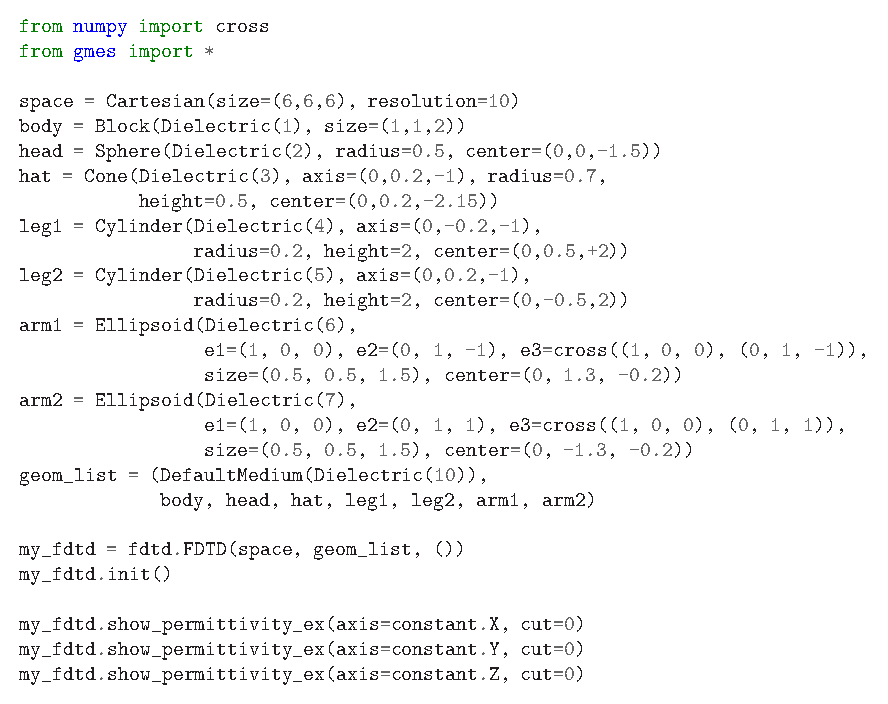
\includegraphics{figure/man}
  \caption{Example of geometric structure representation}
  \label{fig:man_code}
\end{figure}

The first geometric primitive in the geometry list should be \texttt{DefaultMedium} object\index{DefaultMedium class}. This object has infinite dimension, so fills the whole calculation domain. This is to provides a default medium to the calculation domain. A position always belongs to the \texttt{DefaultMedium} object\index{DefaultMedium class}, if it is not belongs to any other primitives in the geometry list.

\texttt{FDTD} and its descendant classes provides a way to check the distribution of the material (or geometric structure) visually. Even the calculation domain is 3 dimension, the display shows just a 2-dimensional display on some cut plane. Figure \ref{fig:man_code} shows how to set this cut plane, and figure \ref{fig:man_perm_view} shows the resulting display.

\begin{figure}[hp!]
  \begin{center}
    \subfigure[]{
      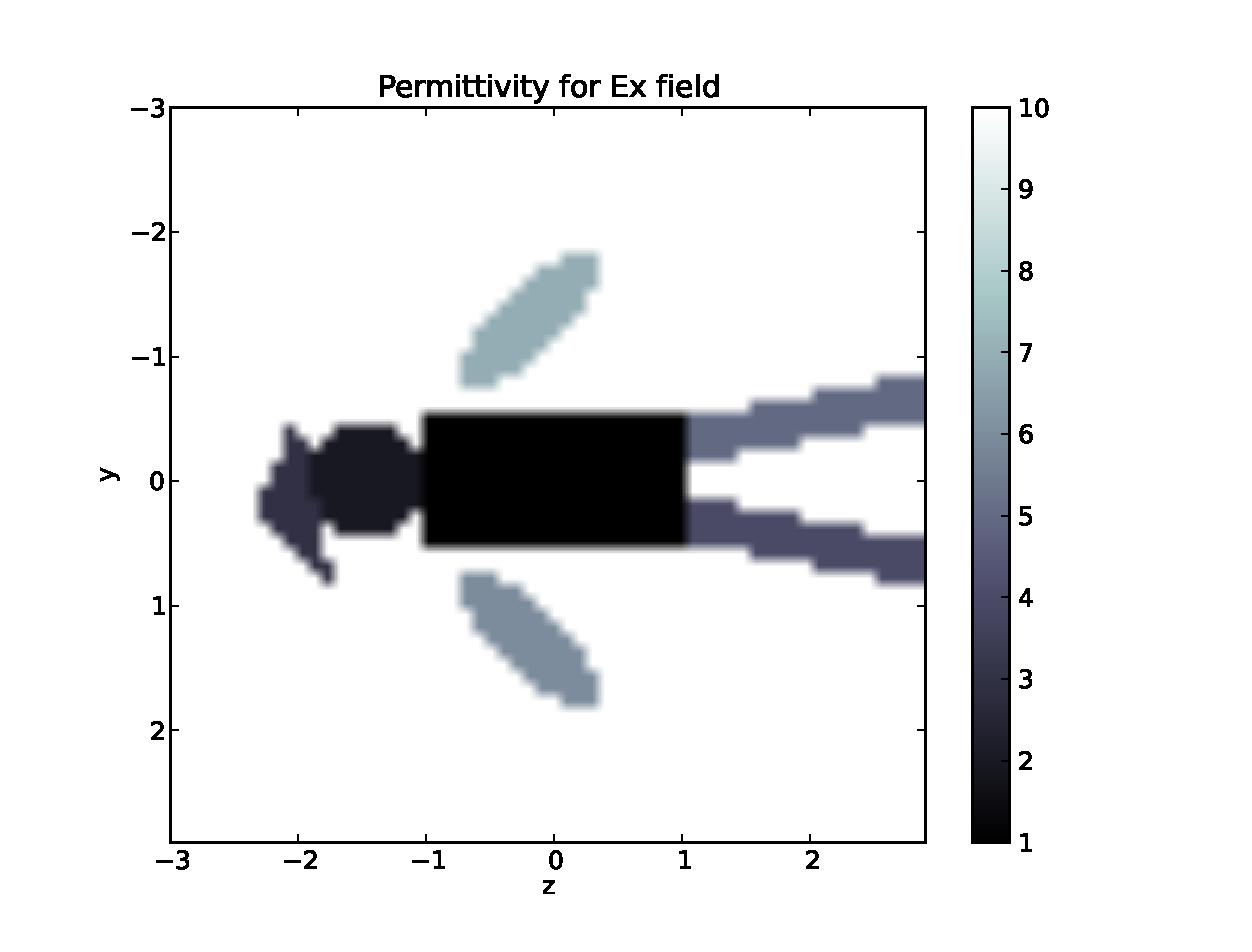
\includegraphics[width=0.45\textwidth]{figure/man_x}
      \label{fig:man_x}
    }
    \subfigure[]{
      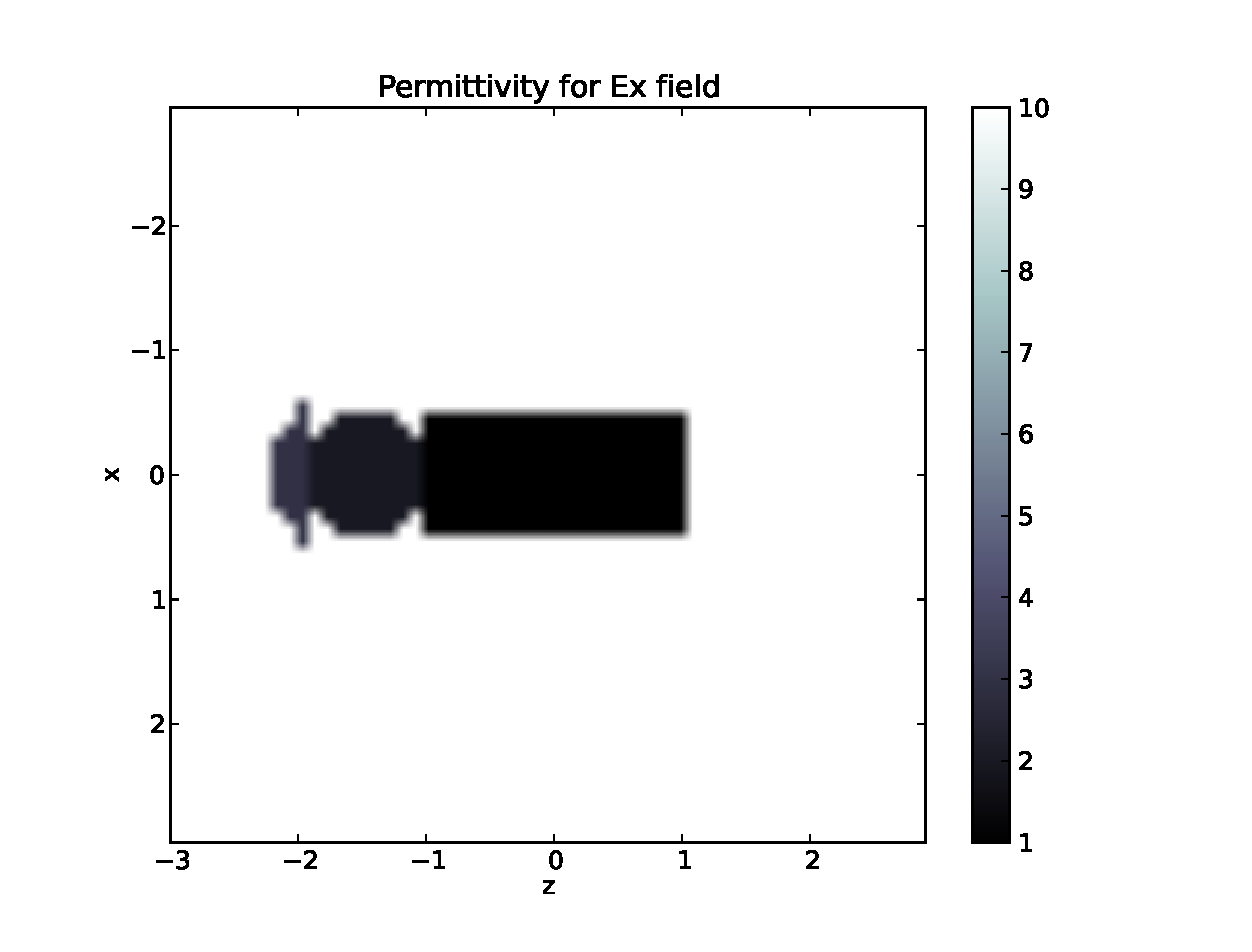
\includegraphics[width=0.45\textwidth]{figure/man_y}
      \label{fig:man_y}
    }
    \subfigure[]{
      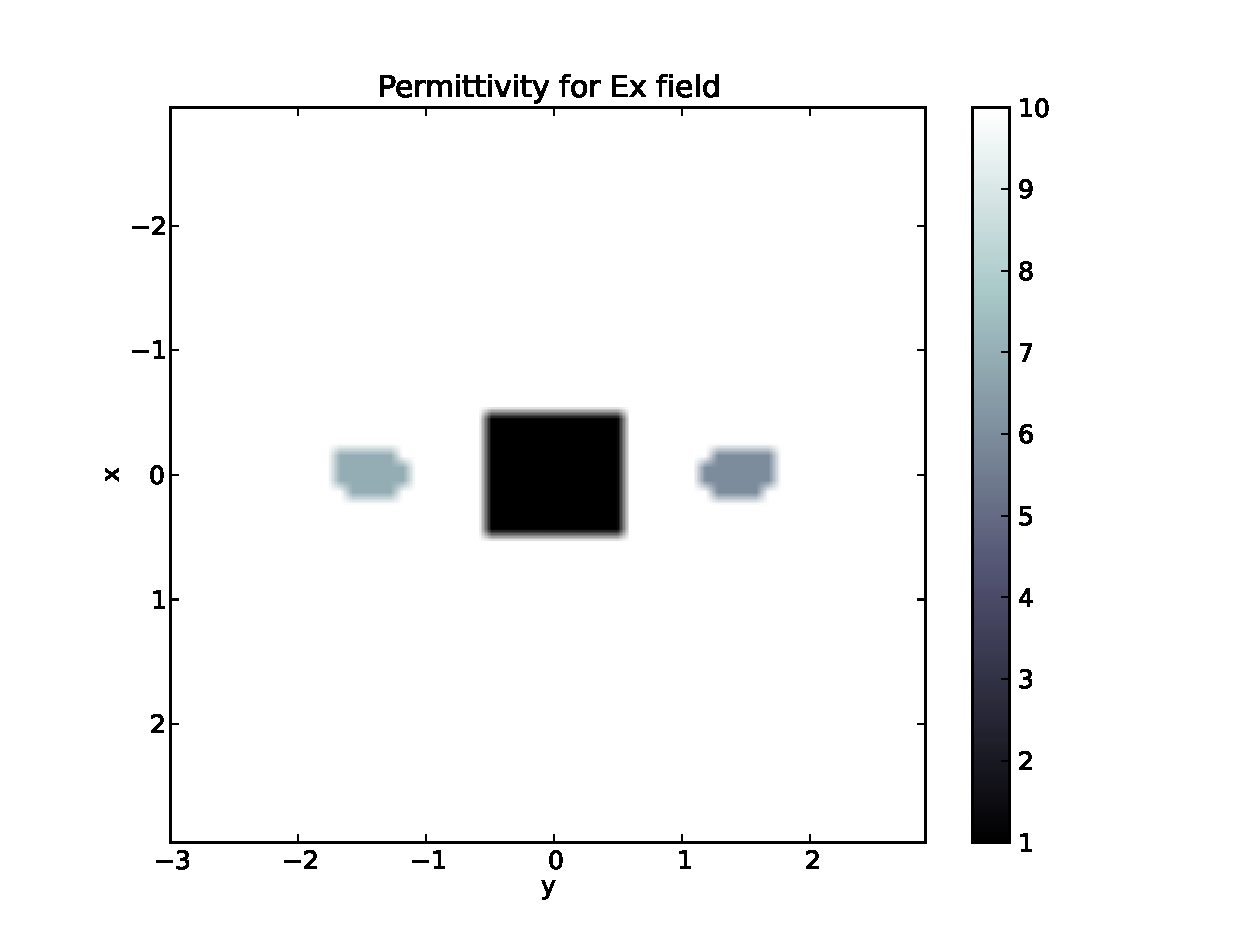
\includegraphics[width=0.45\textwidth]{figure/man_z}
      \label{fig:man_z}
    }
  \end{center}
  \caption{Permittivity distribution displays for $E_x$ field in (a) $x$, (b) $y$, and (c) $z$ planes}
  \label{fig:man_perm_view}
\end{figure}

\section{The plane-wave source condition}
The TF/SF source provides a way to set a plane-wave in a certain zone of a calculation domain. This zone is called a total field zone, because if a scatterer is placed in this zone, the incident field exists along with the scattered field in this zone. On the other hand, the outside of this zone is called scattered field zone, because only scattered field by the object exists. The incident field is removed at the zone interface by the proper adding and subtracting of fields. Figure \ref{fig:tfsf_ex_code} shows the use of TF/SF source.

\begin{figure}
  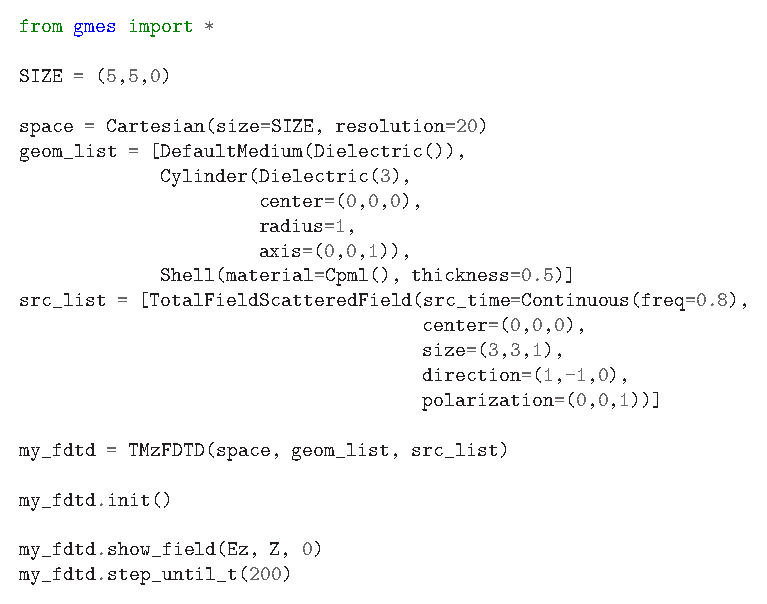
\includegraphics{figure/tfsf_ex_code}
  \caption{An example which shows the usage of the tf/sf source.}
  \label{fig:tfsf_ex_code}
\end{figure}

The tf/sf source is supported by the \texttt{TotalFieldScatteredField} class. This class requires some parameters to set up the zone boundary and plane wave properly. The zone boundary are set to be a rectangular parallelepiped centered at \texttt{center} with \texttt{size}. The consistency condition is set to the plane wave propagating to \texttt{direction} with \texttt{polarization}. The temporal amplitude of the wave is set by the \texttt{SrcTime} object, given to the value of \texttt{src\_time}.

\section{A Bragg-grating-shaped high-pass filter of photonic crystal waveguides}
GMES\index{GMES} can be used for a simulation of a device based on the photonic crystals\index{photonic crystals} (PhC\index{PhC}). This chapter demonstrates an example of it. PhC is consisting of periodic structure of refractive index with period of wavelength of a light. By adjusting the periodicity and refractive index variance, we can make a bandgap\index{bandgap} which prohibits the propagation of the light with certain frequency through the PhC. Using this bandgap as a reflecting mirror and a defect as a light propagating core, we can make a waveguide in the PhC. This waveguide can have a wide bandwidth caused by the wide bandgap of PhC, therefore we can expect multiple channels for the waveguide. We will demonstrate a technique to select a channel among the multiple channels inspired by the Bragg-grating filter of an optical fiber.

For the convenience of the design, A 2-dimensional PhC with dielectric rods in rectangular structures was used, because it has a wide bandgap. Alumina\index{alumina} ($\epsilon_r=8.9$) rods with radius $r=0.2a$ where $a$ is lattice constant $a$ in the air ($\epsilon_r=1$) formed a 2-dimensional PhC. By removing the rods in a line, we made a line defect in this PhC which will be used as a waveguide using the bandgap between the first and second modes of the PhC. Finally, we placed additional dielectric rods in this line defect to make a Bragg-grating structure. If we assume that the structure is one dimension, we can calculate the relation between period of the grating and radius of the rods by
\begin{equation}
\frac{r_B}{a_B} = \frac{1}{\pi} \arcsin \left( k \frac{\Delta \omega}{\omega} \frac{\epsilon_r}{\Delta \epsilon_r} \right)
\label{eq:bragg}
\end{equation}
where $r_B$, $a_B$, $\epsilon_r$, and $\Delta \epsilon_r$ are radius, lattice constant, relative electric permittivity and permittivity difference from the host medium which form the Bragg grating, respectively. Also, $\omega_m$ and $\Delta \omega$ are, respectively, the center frequency and bandwidth of the bandgap and was obtained by the planewave expansion method. The band diagarm of the PhC structure is shown at figure \ref{fig:banddiagram}. $k$ is a proportional constant and set to 0.241788 according to the simulation of 1-dimensional grating. Using Eq.~(\ref{eq:bragg}), The radius of cylinder for the filter with center frequency of 0.35 and 0.48, and bandwidth of 0.2 is $r_B=0.0623302a_B$ and $r_B=0.0362054a_B$, respectively. Each Bragg-gratings are used for high-pass and low-pass filters\index{high-pass filter}\index{low-pass filter}. The PhC waveguide with Bragg grating is shown at figure \ref{fig:phc_waveguide_view}.

\begin{figure}[hp!]
  \centering
  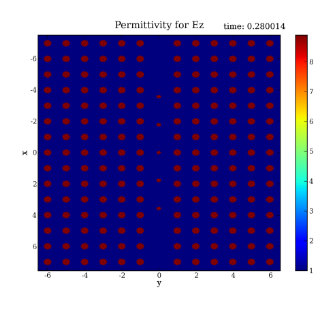
\includegraphics[width=0.8\textwidth]{figure/phc_waveguide_view}
  \caption{2 dimensional PhC waveguide with Bragg-shaped grating}
  \label{fig:phc_waveguide_view}
\end{figure}

The 2-dimensional PhC consisting of rectangular lattice\index{rectangular lattice} with dielectric rods only has bandgap for the transverse magnetic (TM) mode as shown in figure \ref{fig:banddiagram}. Therefore, the simulation had been performed using TM mode 2-dimensional setup of GMES\index{GMES}. The frequency response of the designed filter is shown at figure \ref{fig:freq_response_of_filter}. The low-pass filter does not work well as expected, however, the high-pass filter showed that it reflect the mode in the frequency of 0.32-0.40. We guess that the poor characteristic low-pass filter is caused by too small radius of the rods. Figure \ref{fig:sim_filter_1} and figure \ref{fig:sim_filter_2} shows the propagation of the mode through the high-pass filter. The frequency of the mode is 0.37 and 0.42, respectively.

\begin{figure}[hp!]
  \centering
  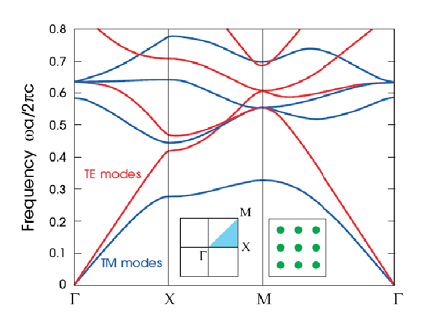
\includegraphics[width=0.8\textwidth]{figure/banddiagram}
  \caption{Band diagram of the PhC consisting of alumina ($\epsilon_r=8.9$) rods with square lattice \cite[p. 80]{joannopoulos_photonic_2008}.}
  \label{fig:banddiagram}
\end{figure}

\begin{figure}[hp!]
  \centering
  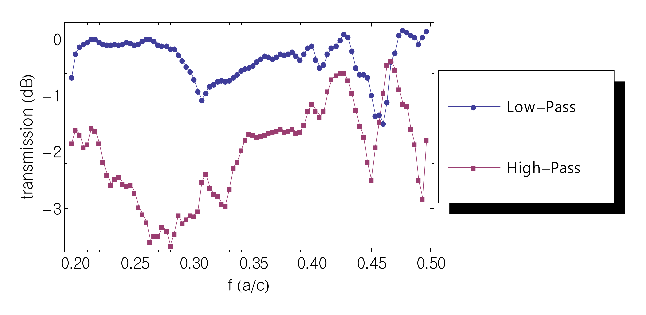
\includegraphics[width=\textwidth]{figure/freq_response_of_filter}
  \caption{Transmission coefficients of high-pass and low-pass filters}
  \label{fig:freq_response_of_filter}
\end{figure}

\begin{figure}[hp!]
  \begin{center}
    \subfigure[$f=0.37$]{
      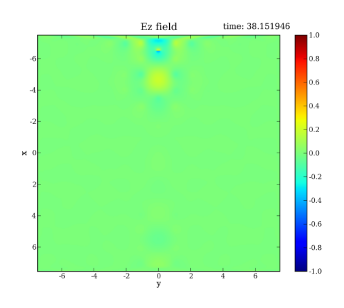
\includegraphics[width=0.5\textwidth]{figure/sim_filter_1}
      \label{fig:sim_filter_1}
    }
    \subfigure[$f=0.42$]{
      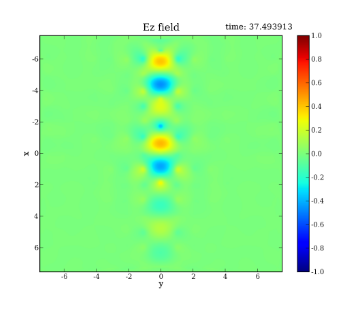
\includegraphics[width=0.5\textwidth]{figure/sim_filter_2}
      \label{fig:sim_filter_2}
    }
  \end{center}
  \caption{Field plots of the propagating waves through the filter.}
  \label{fig:sim_filter}
\end{figure}

We could select a channel of a multi-channel waveguide consisting of PhC, using a Bragg-grating-like structure. By the demonstration, it was shown that a traditional way of Bragg-grating design could be applied to the grating-shaped filter in the PhC waveguide.
